\documentclass[11pt, twocolumn]{article}

\usepackage[spanish]{babel}
\usepackage[none]{hyphenat}
\usepackage[left=1.2cm, right=1.2cm, top = 2cm, bottom=2.5cm]{geometry}
% \usepackage{setspace}
\usepackage{parskip}
\usepackage[export]{adjustbox}
\usepackage{enumitem}
\usepackage{listingsutf8}
\usepackage[dvipsnames]{xcolor}
\usepackage{fancyhdr}
\usepackage{graphicx}
\usepackage{caption}
% \usepackage{subcaption}
% \usepackage{wrapfig}
% \usepackage{multirow, makecell}
% \usepackage{float}
% \usepackage{amsmath} 
% \usepackage{amsfonts}
\usepackage[hidelinks]{hyperref}
\usepackage{csquotes}

\newcommand{\linejump}{\hfill \break}
\renewcommand{\thefootnote}{\fnsymbol{footnote}}
% \newcommand{\unit}[1]{\ensuremath{\, \mathrm{#1}}}

\definecolor{dkgreen}{rgb}{0,0.6,0}
\definecolor{gray}{rgb}{0.5,0.5,0.5}
\definecolor{mauve}{rgb}{0.58,0,0.82}
\lstset{
  language=Java,
  aboveskip=3mm,
  belowskip=3mm,
  showstringspaces=false,
  columns=flexible,
  basicstyle={\tiny\ttfamily},
  numbers=none,
  numberstyle=\tiny\color{gray},
  keywordstyle=\color{blue},
  commentstyle=\color{dkgreen},
  stringstyle=\color{mauve},
  breaklines=true,
  breakatwhitespace=true,
  tabsize=2
}

\sloppy
\setlength{\parindent}{0cm}
\setlength{\columnsep}{0.5cm}
\decimalpoint
\graphicspath{{img/}}

\hypersetup{colorlinks=true, urlcolor=blue, citecolor=blue}
\urlstyle{same}

\pagestyle{fancyplain}
\fancyhf{}
\fancyhead[L]{\scriptsize 
  Universidad Nacional Autónoma de México \\
  Laboratorio de Programación Orientada a Objetos \\
  M.C. Leonardo Ledesma Dominguez
}
\fancyhead[R]{\thepage}

\begin{document}
  \twocolumn[
    \centering
    Acosta Porcayo Alan Omar, Gutiérrez Grimaldo Alejandro, Medina Villa Samuel

    \linejump

    \textbf{\LARGE{Práctica 9. UML}} \\
    
    \linejump
  ]
      
  \footnotetext{
    \scriptsize 
    Acosta Porcayo Alan Omar Ing. en Computación 320206102 \\
    Gutiérrez Grimaldo Alejandro Ing. en Computación 320282098 \\
    Medina Villa Samuel Ing. en Computación 320249538
  }
        
  \fancyfoot{}

  \section*{Resumen}
  En el desarrollo de esta práctica es utilizar UML como una herramienta de diseño para soluciones de \textit{software} en el contexto de programación orientada a objetos. Para lograrlo, se plantea la selección de los diagramas necesarios que mejor representen la solución a un problema dado, seguido por la creación de dichos diagramas UML. Lo que se busca es emplear UML como una herramienta efectiva para diseñar soluciones seleccionando y creando los diagramas apropiados para representar la solución de un problema específico.

  Para esto se presentan los diferentes tipos de diagramas UML y sus características que lo conforman.

  \section*{Introducción}
  El Lenguaje de Modelado Unificado (UML) es un lenguaje gráfico que permite visualizar, especificar y documentar cada parte del desarrollo de software. UML se compone de tres bloques generales: Elementos, Relaciones y Diagramas.

  \subsection*{Diseño Estático o de Estructura}
  En el diseño estático, se utilizan tres tipos de diagramas UML:
  \begin{enumerate}
    \item \textbf{Diagrama de Casos de Uso}
    \begin{itemize}
      \item Permite modelar la interacción entre usuarios y el sistema.
      \item Define actores, casos de uso y relaciones (uso, herencia y comunicación).
    \end{itemize}

    \item \textbf{Diagrama de Clases}
    \begin{itemize}
      \item Modela las características de las clases del sistema.
      \item Muestra atributos, métodos y relaciones entre las clases.
    \end{itemize}

    \item \textbf{Diagrama de Objetos}
    \begin{itemize}
      \item Describe instancias generadas a partir de las clases.
      \item Representa objetos y sus relaciones en un momento específico.
    \end{itemize}
  \end{enumerate}

  \subsection*{Diseño Dinámico o de Comportamiento}
  En el diseño dinámico, se emplean tres tipos de diagramas UML:
  \begin{enumerate}
    \item \textbf{Diagrama de Estados}
    \begin{itemize}
      \item Describe las transiciones que un objeto experimenta a lo largo de su vida.
      \item Incluye nodos de entrada y salida, estados y transiciones.
    \end{itemize}

    \item \textbf{Diagrama de Actividades}
    \begin{itemize}
      \item Muestra el flujo de acciones y objetos involucrados en tareas del sistema.
      \item Contiene nodos de entrada y salida, actividades y transiciones.
    \end{itemize}

    \item \textbf{Diagrama de Interacción}
    \begin{itemize}
      \item Representa la comunicación entre objetos y actores en la ejecución de acciones.
      \item Se divide en Diagrama de Secuencia y Diagrama de Comunicación.
    \end{itemize}
  \end{enumerate}

  \subsection*{Diagrama de Secuencia}
  \begin{itemize}
    \item Muestra una interacción secuencial de eventos.
    \item Visualiza objetos participantes y los mensajes intercambiados.
  \end{itemize}

  \subsection*{Diagrama de Comunicación}
  \begin{itemize}
    \item Muestra la interacción entre varios objetos y el orden en que ocurren.
    \item Define la secuencia de mensajes y flujos de ejecución concurrentes.
  \end{itemize}

  Estos tipos de diagramas en UML permiten a los desarrolladores representar tanto los aspectos estructurales como los comportamentales de un sistema, brindando una herramienta integral para el diseño y la documentación en el desarrollo de \textit{software} orientado a objetos.

  \section*{Objetivos}
  \begin{itemize}
    \item Utilizar diagramas de secuencia en UML para visualizar el flujo de datos y las interacciones entre objetos a lo largo de diferentes escenarios de uso, lo que facilita la detección de posibles problemas de diseño.
    \item Utilizar UML para analizar y documentar los requisitos del \textit{software}, incluyendo la identificación de actores, casos de uso y sus relaciones, lo que permite una comprensión completa de las necesidades del sistema.
    \item Utilizar UML como herramienta para diseñar soluciones de \textit{software} para un lenguaje de programación orientado a objetos.
    
  \end{itemize}

  \section*{Resultados}
  \subsection*{Problema 1}
  Agregue el esquema UML que le tocó realizar en la práctica 9 de laboratorio y de una breve explicación.

  \begin{figure}[h!]
    \centering
    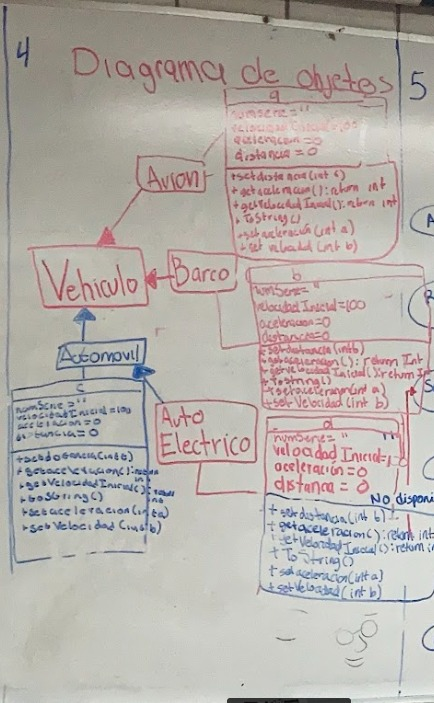
\includegraphics[width=0.56\linewidth]{9P1.jpg}
  \end{figure}

  En el diagrama de objetos hay cuatro objetos: Avión, Barco, Automóvil y Auto Eléctrico. Todos heredan métodos y atributos de la clase Vehículo.

  Hay un objeto llamado Auto Eléctrico que hereda de la clase Automóvil y agrega funcionalidad específica para automóviles eléctricos. El objeto Automóvil hereda métodos y atributos de la clase Vehículo


  \subsection*{Problema 2}
  Seleccione un diagrama UML de otro equipo de laboratorio, anéxelo a su reporte y de una breve explicación.

  \begin{figure}[h!]
    \centering
    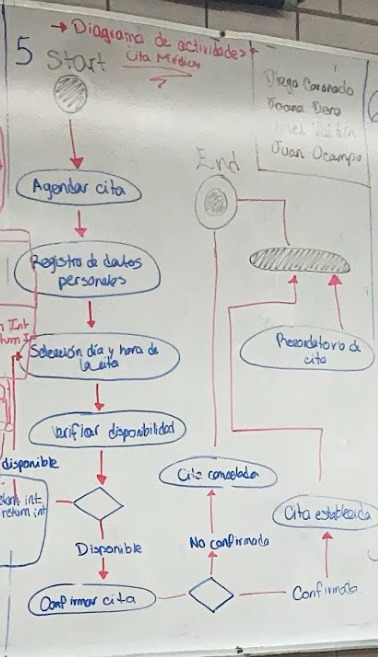
\includegraphics[width=0.6\linewidth]{9P2.jpg}
  \end{figure}

  En el diagrama de actividades es el flujo para poder realizar un cita médica, donde las actividades son: AgendarCita $\longrightarrow$ RegistrarDatosPersonales $\longrightarrow$ SeleccionarDiayHora $\longrightarrow$ , etc.

  Este diagrama de actividades se utiliza para representar visualmente el flujo de actividades, acciones y decisiones, en este caso una cita médica, lo que facilita la comprensión, la comunicación y procesos.

  \section*{Conclusiones}
  Los diagramas UML, conocidos como el Lenguaje de Modelado Unificado, juegan un rol crucial en el proceso de diseño y desarrollo de \textit{software} orientado a objetos. Estas representaciones gráficas desempeñan un papel fundamental al permitirnos visualizar, detallar, registrar y comunicar de manera altamente efectiva tanto los aspectos estructurales como los comportamentales de un sistema.

  A través de una variedad de tipos de diagramas, que incluyen aquellos de casos de uso, clases, objetos, estados, actividades y secuencia, los diseñadores y desarrolladores tienen la capacidad de abordar una amplia diversidad de aspectos en el ciclo de vida del \textit{software}, desde la fase inicial de concepción de requisitos hasta la etapa de implementación y mantenimiento. Estos diagramas no solo actúan como herramientas visuales que facilitan la planificación y el diseño, sino que también se erigen como componentes esenciales en la comunicación efectiva entre los equipos de desarrollo y las partes interesadas del proyecto.

  \twocolumn[
    \centering
    Acosta Porcayo Alan Omar, Gutiérrez Grimaldo Alejandro, Medina Villa Samuel

    \linejump
    
    \textbf{\LARGE{Práctica 10. Excepciones y errores}} \\

    \linejump
  ]

  \section*{Resumen}
  El enfoque de esta práctica es mejorar la calidad y la robustez del código, identificando bloques de código propensos a generar errores y aplicando técnicas apropiadas para el manejo de situaciones excepcionales durante la ejecución. Esto implica la captura de excepciones y errores que puedan surgir en un bloque de código específico. Lo que se busca al realizar este trabajo es fortalecer la integridad del \textit{software} al identificar y gestionar adecuadamente las situaciones imprevistas que podrían afectar su funcionamiento.

  \section*{Introducción}
  La Ley de Pareto, conocida como la regla 80/20, establece que el 80$\%$ de las consecuencias proviene del 20$\%$ de las causas. En el desarrollo de \textit{software}, esto se traduce en que el 80$\%$ del esfuerzo en tiempo y recursos produce el 20$\%$ del código. Además, en términos de calidad, el 80$\%$ de las fallas de una aplicación se generan a partir del 20$\%$ del código. Por lo tanto, la detección y el manejo de errores se convierten en un elemento crucial para asegurar la robustez del \textit{software}.

  Los errores en una aplicación de \textit{software} se pueden clasificar en tres categorías principales:
  \begin{enumerate}
    \item \textbf{Errores Sintácticos:} Estos errores se producen al violar las normas de escritura del lenguaje de programación, como comas mal ubicadas, palabras reservadas escritas de forma incorrecta, entre otros. Por lo general, son detectados por el compilador o el intérprete al procesar el código fuente.
    \item \textbf{Errores Semánticos (o Lógicos):} Los errores semánticos son más sutiles y se presentan cuando la sintaxis del código es correcta, pero la semántica o significado no se ajusta a lo que se pretendía. Estos errores pueden no ser evidentes de inmediato y pueden resultar en un comportamiento incorrecto del programa.
    \item \textbf{Errores de Ejecución:} Estos errores se producen durante la ejecución de la aplicación y pueden deberse al uso incorrecto por parte del usuario (por ejemplo, ingresar una cadena en lugar de un número) o a errores de programación, como acceder a ubicaciones no permitidas en la memoria. Los errores de ejecución provocan la terminación abrupta del programa.
  \end{enumerate}

  Para manejar estos errores en tiempo de ejecución, se utilizan las excepciones. Las excepciones son condiciones excepcionales que alteran el flujo normal del programa y pueden ser generadas tanto por la lógica del programa como por objetos que informan sobre condiciones inesperadas o no manejables.
  
  Las excepciones se dividen en dos grandes grupos:
  \begin{itemize}
    \item \textbf{Excepciones Marcadas:} Estas excepciones requieren que se capturen de manera obligatoria mediante bloques catch en el código.
    \item \textbf{Excepciones No Marcadas:} Las excepciones en tiempo de ejecución (\textit{RuntimeException} y sus subclases) no requieren una captura obligatoria.
  \end{itemize}

  Para manejar las excepciones, se utilizan bloques \textit{try} y \textit{catch}, donde el bloque \textit{try} define la sección del código en la que puede ocurrir una excepción, y el bloque \textit{catch} maneja la excepción arrojada. Los errores que no se manejan pueden propagarse a través de los métodos, y para indicar que un método puede lanzar una excepción, se utiliza la palabra reservada \textit{``throws''}.

  \subsection*{Propagación de Excepciones}
  La propagación de excepciones es el proceso mediante el cual una excepción se transfiere desde el punto donde se genera hasta un punto donde se puede manejar o capturar la excepción. Si una excepción no se maneja en el lugar donde se origina, se propaga hacia arriba en la pila de llamadas de métodos hasta que se encuentra un bloque \textit{``catch''} adecuado para manejarla.

  \subsection*{\textit{Throw}}
  La palabra reservada \textit{``throw''} se utiliza para lanzar o arrojar una excepción de manera explícita en el código. Esto permite a los programadores indicar que ha ocurrido un error o una situación excepcional y que se debe tomar una acción específica para manejarlo

  \subsection*{\textit{Throws}}
  La palabra reservada \textit{``throws''} se utiliza en la firma de un método para indicar que el método puede lanzar excepciones específicas. Esto notifica a quien llama al método que debe manejar o propagar las excepciones mencionadas. 

  \subsection*{Excepciones Propias}
  Las excepciones propias son clases de excepción que se crean específicamente para representar errores o situaciones excepcionales relacionadas con un dominio de negocio particular. Estas clases de excepción suelen heredar de la clase \textit{Exception} o \textit{Throwable} y permiten personalizar el manejo de errores en una aplicación

  \section*{Objetivos}
  \begin{itemize}
    \item Identificar y solucionar bloques de código que puedan causar problemas de usabilidad o errores que afecten negativamente la experiencia del usuario.
    \item Aplicar buenas prácticas de codificación y manejo de excepciones para que el código sea más comprensible y colaborativo
    \item Identificar bloques de código propensos a generar errores y aplicar técnicas adecuadas para el manejo de situaciones excepcionales en tiempo de ejecución    
  \end{itemize}

  \section*{Metodología}
  \textbf{Enumeración \textit{Sx}}
  \begin{lstlisting}
public enum Sx {
  FEMENINO, 
  MASCULINO, 
  INDETERMINADO
};
  \end{lstlisting}

  \textbf{\textit{Persona.java}}
  \begin{lstlisting}
abstract class Persona{
  String nombre;
  int edad;
  Sx sexo;
  String nacionalidad;

  public String getNombre() {
    return this.nombre;
  }

  public int getEdad() {
    return this.edad;
  }

  public Sx getSexo() {
    return this.sexo;
  }

  public String getNacionalidad() {
    return this.nacionalidad;
  }

  abstract boolean votar();
  abstract boolean servicioMilitar();
  abstract boolean serPresidente();
}

class Mexicano extends Persona {
  String curp;
  Mexicano(String nombre, int edad, Sx sexo, String curp) {
    this.nombre=nombre;
    this.sexo=sexo;
    this.edad=edad;
    this.curp=curp;
    this.nacionalidad="Mexicano";
  }

  @Override
  boolean votar(){
    return (this.edad >=18) ?  true : false;
  }

  @Override
  boolean servicioMilitar() {
    return (this.edad >=17 && this.sexo == Sx.MASCULINO) ?  true : false;
  }

  @Override
  boolean serPresidente() {
    return (this.edad >=35) ?  true : false;
  }
}

class Extranjero extends Persona {
  Extranjero(String nombre, int edad, Sx sexo) {
    this.nombre=nombre;
    this.sexo=sexo;
    this.edad=edad;
    this.nacionalidad="Extranjero";
  }

  @Override
  boolean votar() {
    return false;
  }

  @Override
  boolean servicioMilitar() {
    return false;
  }

  @Override
  boolean serPresidente() {
    return false;
  }
}
  \end{lstlisting}

  \section*{\textit{OuterException.java}}
  \begin{lstlisting}
class OuterException extends Exception {
  OuterException(String s) {
    super(s);
  }
  
  OuterException(String s, boolean sth) {
    InnerException2 local = new InnerException2(s);
  }

  static class InnerException extends Exception {
    InnerException(String s) {
      super(s);
    }
  }
  
  class InnerException2 extends Exception {
    
    InnerException2(String s) {
      System.out.println(s);
    }
  }
}    
  \end{lstlisting}

  \textbf{\textit{Principal.java}}
  \begin{lstlisting}
import java.util.HashMap;

class Principal {
  public static void main(String[] args) 
      throws OuterException, OuterException.InnerException {
    HashMap<String,Persona> gente = new HashMap<String,Persona>();

    gente.put("ERZ123220PO",new Mexicano("Eric",19,Sx.MASCULINO, "ERZ123220PO"));
    gente.put("AMZ453220LO",new Mexicano("Amir",19,Sx.INDETERMINADO, "AMZ453220LO"));
    gente.put("ABN123980KO",new Mexicano("Abner",16,Sx.MASCULINO, "ABN123980KO"));
    gente.put("SFN154620JO",new Mexicano("Sofia",19,Sx.FEMENINO, "SFN154620JO"));
    gente.put("IRN135220GO",new Mexicano("Irandy",19,Sx.FEMENINO, "IRN135220GO"));

    gente.forEach((k,p)-> {System.out.println(k + " : Nombre - " 
        + p.getNombre() + " : Edad - " + p.getEdad() );});
    
    //levantar excepcion por no poder votar
    gente.forEach((k, p) -> {
      try {
        if (!p.votar()) 
          throw new OuterException("no puede votar : " + p.getNombre());
      } catch (OuterException n) {
        System.out.println(n);
      }
    });

    gente.forEach((k, p) -> {
      try {
        if (!p.serPresidente()) 
          throw new OuterException.InnerException
              ("no puede ser presidente : " + p.getNombre());
      } catch (OuterException.InnerException n) {
        System.out.println(n);
      }
    });

    gente.forEach((k, p) -> {
        try {
          if (!p.servicioMilitar()) 
            throw new OuterException
                ("no puede realizar su servicio militar : " + p.getNombre(), true);
        } catch (OuterException n) {
          return;
        }
    });
  }
}    
  \end{lstlisting}

  \section*{Resultados}
  \subsection*{Problema 1}
  Modifique el programa visto durante la práctica para construir objetos ``Persona'' desde consola solicitando nombre, edad, nacionalidad y sexo, la llave CURP.

  \textbf{\textit{Principal.java}}
  \begin{lstlisting}
import java.util.HashMap;
import java.util.Scanner;

class Principal {
	public static void main(String[] args) throws OuterException,
      OuterException.InnerException {
		HashMap<String,Persona> gente = new HashMap<String,Persona>();
		Scanner sc = new Scanner(System.in);

		while(true) {
			System.out.print("Ingrese el nombre: ");
			String nombre = sc.next();
			System.out.print("Ingrese la edad: ");
			int edad = sc.nextInt();
			System.out.print("Ingrese el sexo: ");
			Sx sexo = Sx.valueOf(sc.next().toUpperCase());
			System.out.print("Ingrese el CURP: ");
			String curp = sc.next();

			gente.put(curp,new Mexicano(nombre,edad,sexo,curp));
			
			System.out.println("Desea agregar otra persona? (s/n)");
			String resp = sc.next();
			if(resp.equals("n")) 
				break;
			System.out.println(" ");
		}

		gente.forEach((k,p)-> {System.out.println(k + " : Nombre - " 
        + p.getNombre() + " : Edad - " + p.getEdad() );});

		gente.forEach((k, p) -> {
		try {
			if (!p.votar()) 
			throw new OuterException("no puede votar : " + p.getNombre());
		} catch (OuterException n) {
			System.out.println(n);
		}
		});

		gente.forEach((k, p) -> {
		try {
			if (!p.serPresidente()) 
			throw new OuterException.InnerException
				("no puede ser presidente : " + p.getNombre());
		} catch (OuterException.InnerException n) {
			System.out.println(n);
		}
		});

		gente.forEach((k, p) -> {
			try {
				if (!p.servicioMilitar()) 
				throw new OuterException
					("no puede realizar su servicio militar : " + p.getNombre(), true);
			} catch (OuterException n) {
				return;
			}
		});

		sc.close();
	}
}
  \end{lstlisting}

  \newpage
  \textbf{Ejecución}
  \begin{figure}[h!]
    \centering
    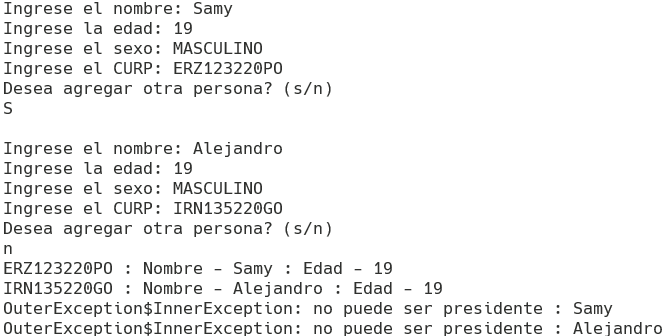
\includegraphics[width=0.9\linewidth]{10P1.png}
  \end{figure}

  \subsection*{Problema 2}
  Revise el siguiente código ubicado en: \url{https://howtodoinjava.com/java/exception-handling/best-practices-for-for-exception-handling/}

  Implemente el punto 2 del blog utilizando la misma lógica para controlar excepciones:

  \begin{enumerate}[label=\alph*)]
    \item Un extranjero no puede ser mexicano, al momento de ser creado.
    \item Construya una excepción que no permita crear Personas con edad $<=$ 0 años.
    \item Construya una excepción que permita jubilar a una Persona considere la edad de jubilación de $>=$ 64 años.
  \end{enumerate}
  
  \textbf{\textit{Persona.java}}
  \begin{lstlisting}
  abstract class Persona {
	String nombre;
	int edad;
	Sx sexo;
	String nacionalidad;

	public String getNombre() {
		return this.nombre;
	}

	public int getEdad() {
		return this.edad;
	}

	public Sx getSexo() {
		return this.sexo;
	}

	public String getNacionalidad() {
		return this.nacionalidad;
	}

	abstract boolean votar();

	abstract boolean servicioMilitar();

	abstract boolean serPresidente();

	public void verificarNacionalidad() 
			throws NacionalidadInvalidaException {
		if (this.nacionalidad.equals("Mexicano") && this instanceof Extranjero) {
			throw new 
          NacionalidadInvalidaException("Un extranjero no puede ser mexicano.");
		}
	}

	public void verificarEdad() throws EdadInvalidaException {
		if (this.edad <= 0) {
			throw new 
          EdadInvalidaException("La edad no puede ser menor o igual a 0.");
		}
	}

	abstract boolean jubilar() throws JubilacionException;

	public void verificarJubilacion() throws JubilacionException {
		if (this.edad < 64) {
			throw new 
          JubilacionException("La persona no cumple con la edad minima para jubilarse.");
		}
	}
}

class Mexicano extends Persona {
	String curp; 

	Mexicano(String nombre, int edad, Sx sexo, String curp) {
		this.nombre = nombre;
		this.sexo = sexo;
		if (edad <= 0) {
			throw new 
          EdadInvalidaException("La edad no puede ser menor o igual a 0.");
		}
		this.edad = edad;
		this.curp = curp;
		this.nacionalidad = "Mexicano";
	}

	@Override
	boolean votar() {
		return (this.edad >= 18) ? true : false;
	}

	@Override
	boolean servicioMilitar() {
		return (this.edad >= 17 && this.sexo == Sx.MASCULINO) ? true : false;
	}

	@Override
	boolean serPresidente() {
		return (this.edad >= 35) ? true : false;
	}

	@Override
	boolean jubilar() throws JubilacionException {
		verificarJubilacion();
		return true;
	}
}

class Extranjero extends Persona {
	Extranjero(String nombre, int edad, Sx sexo) {
		this.nombre = nombre;
		this.sexo = sexo;
		if (edad <= 0) {
			throw new 
          EdadInvalidaException("La edad no puede ser menor o igual a 0.");
		}
		this.edad = edad;
		this.nacionalidad = "Extranjero";
	}

	@Override
	boolean votar() {
		return false;
	}

	@Override
	boolean servicioMilitar() {
		return false;
	}

	@Override
	boolean serPresidente() {
		return false;
	}

	@Override
	boolean jubilar() throws JubilacionException {
		verificarJubilacion();
		return true;
	}
}
  \end{lstlisting}

  \textbf{\textit{OuterException.java}}
  \begin{lstlisting}
class OuterException extends Exception {
	OuterException(String s) {
		super(s);
	}

	OuterException(String s, boolean sth) {
		InnerException2 local = new InnerException2(s);
	}

	static class InnerException extends Exception {
		InnerException(String s) {
			super(s);
		}
	}

	class InnerException2 extends Exception {

		InnerException2(String s) {
			System.out.println(s);
		}
	}
}

class NacionalidadInvalidaException extends Exception {
	public NacionalidadInvalidaException(String message) {
		super(message);
	}
}

class EdadInvalidaException extends IllegalArgumentException {
	public EdadInvalidaException(String message) {
		super(message);
	}
}

class JubilacionException extends Exception {
	public JubilacionException(String message) {
		super(message);
	}
}
  \end{lstlisting}

  \textbf{Ejecución}
  \begin{figure}[h!]
    \centering
    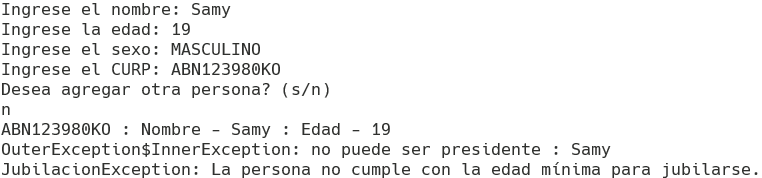
\includegraphics[width=\linewidth]{10P2.png}
  \end{figure}

  \subsection*{Problema 3}
  Usando instrucciones \textit{try-catch} aplique la jerarquía de excepciones de la siguiente manera:

  \begin{enumerate}
    \item Es mexicano
    \item Puede Votar
    \item Puede ser presidente
  \end{enumerate}

  Considerando que la 1 es la de mas alta prioridad y podrá acceder al nivel 2 y así sucesivamente.

  \textbf{\textit{Persona.java}}
  \begin{lstlisting}
class NoEsMexicanoException extends Exception {
}

class NoPuedeVotarException extends Exception {
}

class NoPuedeSerPresidenteException extends Exception {
}

abstract class Persona {
	String nombre;
	int edad;
	Sx sexo;
	String nacionalidad;

	public String getNombre() {
		return this.nombre;
	}

	public int getEdad() {
		return this.edad;
	}

	public Sx getSexo() {
		return this.sexo;
	}

	public String getNacionalidad() {
		return this.nacionalidad;
	}

	abstract boolean votar();

	abstract boolean servicioMilitar();

	abstract boolean serPresidente();

	public void verificarNacionalidad()
			throws NoEsMexicanoException, NoPuedeVotarException, 
      NoPuedeSerPresidenteException {
		try {
			if (!this.nacionalidad.equals("Mexicano")) {
				throw new NoEsMexicanoException();
			}

			try {
				if (!this.votar()) {
					throw new NoPuedeVotarException();
				}

				try {
					if (!this.serPresidente()) {
						throw new NoPuedeSerPresidenteException();
					}
				} catch (NoPuedeSerPresidenteException e) {
					System.out.println("Puede votar pero no puede ser presidente");
					throw e;
				}
			} catch (NoPuedeVotarException e) {
				System.out.println("Es mexicano pero no puede votar");
				throw e;
			}
		} catch (NoEsMexicanoException e) {
			System.out.println("No es mexicano");
			throw e;
		}
	}

	public void verificarEdad() throws EdadInvalidaException {
		if (this.edad <= 0) {
			throw new 
          EdadInvalidaException("La edad no puede ser menor o igual a 0.");
		}
	}

	abstract boolean jubilar() throws JubilacionException;

	public void verificarJubilacion() throws JubilacionException {
		if (this.edad < 64) {
			throw new 
          JubilacionException("La persona no cumple con la edad minima para jubilarse.");
		}
	}
}

class Mexicano extends Persona {
	String curp;

	Mexicano(String nombre, int edad, Sx sexo, String curp) {
		this.nombre = nombre;
		this.sexo = sexo;
		if (edad <= 0) {
			throw new 
          EdadInvalidaException("La edad no puede ser menor o igual a 0.");
		}
		this.edad = edad;
		this.curp = curp;
		this.nacionalidad = "Mexicano";
	}

	@Override
	boolean votar() {
		return (this.edad >= 18) ? true : false;
	}

	@Override
	boolean servicioMilitar() {
		return (this.edad >= 17 && this.sexo == Sx.MASCULINO) ? true : false;
	}

	@Override
	boolean serPresidente() {
		return (this.edad >= 35) ? true : false;
	}

	@Override
	boolean jubilar() throws JubilacionException {
		verificarJubilacion();
		return true;
	}
}

class Extranjero extends Persona {
	Extranjero(String nombre, int edad, Sx sexo) {
		this.nombre = nombre;
		this.sexo = sexo;
		if (edad <= 0) {
			throw new 
          EdadInvalidaException("La edad no puede ser menor o igual a 0.");
		}
		this.edad = edad;
		this.nacionalidad = "Extranjero";
	}

	@Override
	boolean votar() {
		return false;
	}

	@Override
	boolean servicioMilitar() {
		return false;
	}

	@Override
	boolean serPresidente() {
		return false;
	}

	@Override
	boolean jubilar() throws JubilacionException {
		verificarJubilacion();
		return true;
	}
}
  \end{lstlisting}

  \textbf{\textit{OuterException.java}}
  \begin{lstlisting}
class OuterException extends Exception {
	OuterException(String s) {
		super(s);
	}

	OuterException(String s, boolean sth) {
		InnerException2 local = new InnerException2(s);
	}

	static class InnerException extends Exception {
		InnerException(String s) {
			super(s);
		}
	}

	class InnerException2 extends Exception {

		InnerException2(String s) {
			System.out.println(s);
		}
	}
}

class NacionalidadInvalidaException extends Exception {
	public NacionalidadInvalidaException(String message) {
		super(message);
	}
}

class EdadInvalidaException extends IllegalArgumentException {
	public EdadInvalidaException(String message) {
		super(message);
	}
}

class JubilacionException extends Exception {
	public JubilacionException(String message) {
		super(message);
	}
}
  \end{lstlisting} 

  \textbf{\textit{Principal.java}}
  \begin{lstlisting}
import java.util.HashMap;
import java.util.Scanner;

class Principal {
	public static void main(String[] args)
			throws OuterException, OuterException.InnerException {
		HashMap<String, Persona> gente = new HashMap<String, Persona>();
		Scanner sc = new Scanner(System.in);

		while (true) {
			System.out.print("Ingrese el nombre: ");
			String nombre = sc.next();
			System.out.print("Ingrese la edad: ");
			int edad = sc.nextInt();
			System.out.print("Ingrese el sexo: ");
			Sx sexo = Sx.valueOf(sc.next().toUpperCase());
			System.out.print("Ingrese el CURP: ");
			String curp = sc.next();

			gente.put(curp, new Mexicano(nombre, edad, sexo, curp));

			System.out.println("Desea agregar otra persona? (s/n)");
			String resp = sc.next();
			if (resp.equals("n"))
				break;
			System.out.println(" ");
		}

		gente.forEach((k, p) -> {
			System.out.println(k + " : Nombre - "
					+ p.getNombre() + " : Edad - " + p.getEdad());
		});

		gente.forEach((k, p) -> {
			try {
				if (!p.votar())
					throw new 
						OuterException("no puede votar : " + p.getNombre());
			} catch (OuterException n) {
				System.out.println(n);
			}
		});

		gente.forEach((k, p) -> {
			try {
				if (!p.serPresidente())
					throw new 
						OuterException.InnerException("no puede ser presidente : " + p.getNombre());
			} catch (OuterException.InnerException n) {
				System.out.println(n);
			}
		});

		gente.forEach((k, p) -> {
			try {
				if (!p.servicioMilitar())
					throw new 
						OuterException("no puede realizar su servicio militar : " + p.getNombre(), true);
			} catch (OuterException n) {
				return;
			}
		});

		gente.forEach((k, p) -> {
			try {
				if (!p.jubilar())
					throw new 
						JubilacionException("no puede jubilarse : " + p.getNombre());
			} catch (JubilacionException n) {
				System.out.println(n);
			}
		});

		sc.close();
	}
}
  \end{lstlisting}

  \section*{Conclusiones}
  Las excepciones y los errores desempeñan un papel fundamental en el desarrollo de \textit{software} y la programación en general. Son un componente esencial para garantizar la confiabilidad, la robustez y la calidad de los programas. El manejo de excepciones nos permite controlar y gestionar situaciones excepcionales de manera predecible en lugar de permitir que los errores provoquen fallos inesperados o la terminación abrupta de un programa. Todo esto con el fin de contribuir a la mejora de la calidad del código y a prevenir problemas futuros.

  \begin{enumerate}
    \item Sin modificar el programa original, dejaría de funcionar el programa si quitamos la instrucción \textit{throws} de la clase \textit{Principal}. ¿si por qué o no por qué?
    
    Quitando la instrucción \textit{throws} de la clase \textit{Principal}, el programa no dejaría de funcionar debido a que las posibles excepiones dentro del codigo estan siendo controladas por bloques \textit{try-catch}, de manera que \textit{throws} no es necesario para el funcionamiento del programa.

    \item Indique cuál es la ventaja de usar \textit{inner class} genéricas y cuál es la ventaja de usar \textit{static inner class}.
    
    \subsubsection*{Ventajas de usar clases internas genéricas}
    Las clases internas genéricas ofrecen la posibilidad de crear componentes reutilizables que pueden funcionar con una variedad de tipos de datos sin necesidad de duplicar el código. Esta característica fomenta la reutilización y la modularidad en el desarrollo de software.

    El uso de tipos genéricos garantiza un código más seguro y menos propenso a errores, ya que el compilador realiza verificaciones de tipo durante la compilación, lo que previene errores de tipo en tiempo de ejecución.

    Las clases internas genéricas son adaptables a diferentes tipos de datos, lo que las hace versátiles y adecuadas para la implementación de estructuras de datos genéricas, como colecciones, árboles, pilas y otras estructuras similares.

    \subsubsection*{Ventajas de usar clases internas estáticas}
    Las clases internas estáticas no precisan de una instancia de la clase externa para su instanciación, lo que implica que se pueden utilizar sin requerir la creación de una instancia de la clase contenedora, lo cual puede resultar en ahorro de recursos.

    Frecuentemente, las clases internas estáticas se emplean para encapsular funcionalidades compartidas por todas las instancias de la clase externa, evitando así la duplicación de código y promoviendo la eficacia en el desarrollo.

    Debido a su naturaleza estática, estas clases internas no tienen acceso a las variables de instancia de la clase contenedora, lo que contribuye a prevenir problemas de concurrencia y a mejorar el rendimiento en aplicaciones multihilo.
    
    \item Porque las excepciones en JAVA de tipo no marcadas no pueden ser únicamente
    \textit{\textbf{RunTime Exception}}.

    Las excepciones en Java de tipo no marcadas no son únicamente \textit{RuntimeException}, ya que también pueden ser otras excepciones no marcadas, como \textit{NullPointerException}, \textit{ArrayIndexOutOfBoundsException}, \textit{IllegalArgumentException}, entre otras. Las excepciones no marcadas representan errores en tiempo de ejecución que no necesitan ser declarados en la firma de un método, pero aún deben manejarse apropiadamente para evitar problemas en la aplicación.
  \end{enumerate}

  \section*{Referencias}
  \begin{small}
    Gupta, L., $\&$ Gupta, L. (2023, April 7). \textit{Effective approach for creating custom exceptions in Java}. HowToDoInJava. \url{https://howtodoinjava.com/java/exception-handling/best-practices-for-for-exception-handling/} \\

    Solano, J. (2017, 20 enero). \textit{Manual de prácticas de Programación Orientada a Objetos}. Laboratorio de Computación Salas A y B. \url{http://lcp02.fi-b.unam.mx/} \\
  \end{small}
\end{document}